\documentclass[review]{elsarticle}

\usepackage{lineno,hyperref}
\usepackage{xcolor}
\usepackage[labelfont=bf]{caption}
\modulolinenumbers[5]

\bibliographystyle{elsarticle-num}

\newcommand{\beginsupplement}{%
        \setcounter{table}{0}
        \renewcommand{\thetable}{S\arabic{table}}%
        \setcounter{figure}{0}
        \renewcommand{\thefigure}{S\arabic{figure}}%
     }

\begin{document}

\begin{frontmatter}

\title{SUPPLEMENTARY MATERIAL FOR: \newline
Investigating Facebook's interventions against accounts that repeatedly share misinformation}

\author[mymainaddress]{Héloïse Théro\corref{mycorrespondingauthor}}
\cortext[mycorrespondingauthor]{Corresponding authors.}
\ead{thero.heloise@gmail.com}

\author[mymainaddress]{Emmanuel M. Vincent}
\ead{emmanuel.vincent@sciencespo.fr}

\address[mymainaddress]{médialab - Sciences Po, Paris, France}

\begin{abstract}

Further analysis of repeat offenders' engagement metrics, and overlap between Science Feedback and Condor datasets.

\end{abstract}

\end{frontmatter}

\beginsupplement

\section*{Engagement dynamics plotted separately for groups and pages}

In this article, we find that Facebook groups and pages are affected differently by Facebook’s policies against misinformation.
The timeseries of engagement metrics shown in Figures 3 and 6, include both groups and pages as they intend to represent the overall engagement that repeat offenders accounts are able to generate on Facebook.

However, since the `June drop’ is only affecting Facebook groups and not pages, we display the timeseries of engagement per post separately for groups and pages below. See Figure \ref{engagement_groups_and_pages_sf} for the accounts identified using the Science Feedback dataset and Figure \ref{engagement_groups_and_pages_condor} for the accounts identified using the Condor dataset. 
We observe that the engagement per post drops for `repeat offender' groups in June 2020 while it does not for pages.

Figure \ref{engagement_groups_and_pages_reduce} displays the timeseries of engagement per post for the set of pages that shared a `reduced distribution' notification.
As with the sets of pages shown above, there is no reduction in engagement for these pages in June 2020.

\begin{figure}[!h]
\centering
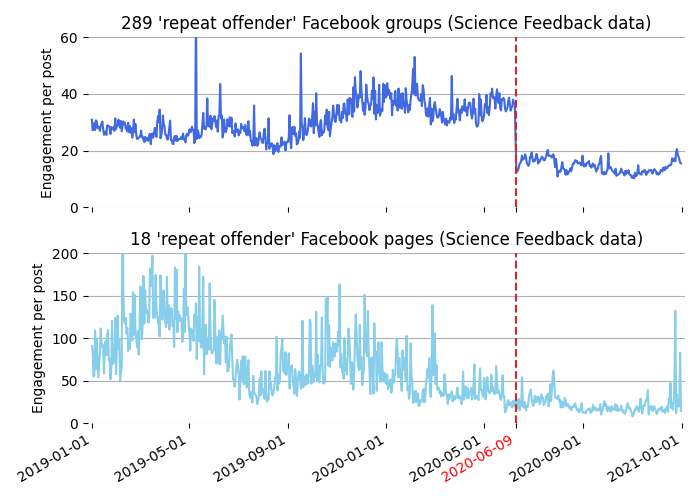
\includegraphics[scale=0.5]{./../figure/supplementary_engagement_groups_and_pages_sf.png}
\caption{
Average engagement per post in 2019-2020 plotted separately for the 289 groups (top panel) and the 18 pages (bottom panel) identified as `repeat offender' using Science Feedback data.
}
\label{engagement_groups_and_pages_sf}
\end{figure}

\begin{figure}[!h]
\centering
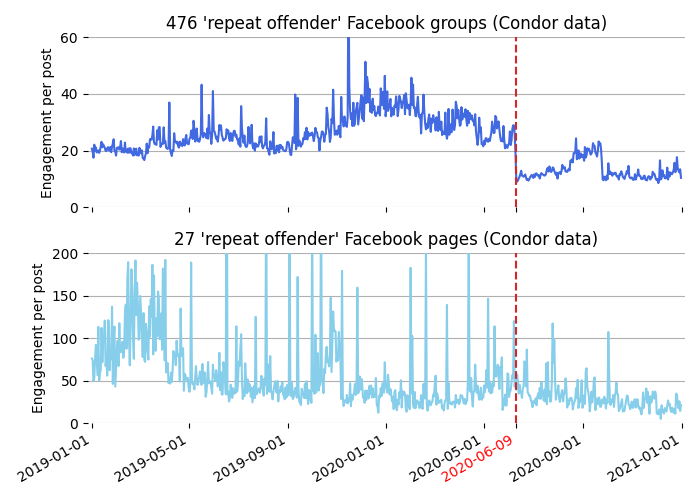
\includegraphics[scale=0.5]{./../figure/supplementary_engagement_groups_and_pages_condor.png}
\caption{
Average engagement per post in 2019-2020 plotted separately for the 476 groups (top panel) and the 27 pages (bottom panel) identified as `repeat offender' using Condor data.
}
\label{engagement_groups_and_pages_condor}
\end{figure}

\begin{figure}[!h]
\centering
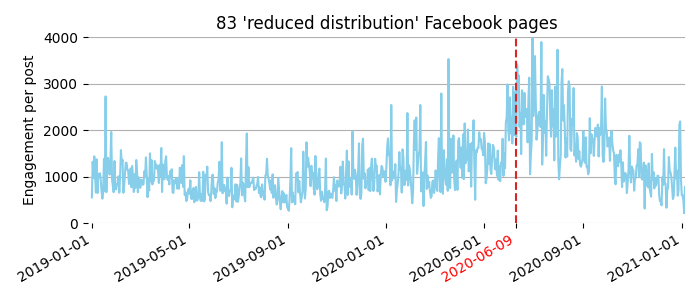
\includegraphics[scale=0.5]{./../figure/supplementary_engagement_pages_reduce.png}
\caption{
Average engagement per post in 2019-2020 for the 80 `reduced distribution' pages, identified because they shared a `reduced distribution' notification from Facebook.
}
\label{engagement_groups_and_pages_reduce}
\end{figure}

These graphs illustrate that only Facebook groups, and not pages, were affected by the reduce measure implemented on June 9, 2020.

\section*{Engagement dynamics in 2019-2020 for a control set of accounts}

To ensure that the engagement metrics changes we observed specifically affect repeat offender accounts, we compare their dynamics to those of a control set of accounts, which consist of Facebook pages and groups associated with established news outlets that we expect to have a more stable pattern of publishing and represent the baseline journalistic activity. 

To identify such a set, we used a report from NewsWhip \citep{NewsWhipReport} that identified the 10 media outlets that communicated the most during the early phase of the COVID-19 pandemic (first half of 2020), i.e., NBC, The Daily Mail, CNN, Fox News, The Independent, BBC, The New York Times, The Washington Post, Yahoo and The New York Post.
We searched the outlets' names on Facebook and created a list of 10 pages and six groups that displayed a verified `blue check'.
We also searched for more groups as they are the accounts supposed to be affected by the June drop.
In addition to these, and since  groups are the only type of accounts potentially affected by the `June drop', we searched for additional groups that focus on sharing information on scientific topics (searching for keywords related to health, vaccines or climate change) and that did not get flagged for sharing URLs marked as false.
We identified 19 additional Facebook groups created before June 2020.
Using CrowdTangle, we collected all the posts published by these accounts between January 1, 2019 and December 31, 2020.

\begin{figure}[!h]
\centering
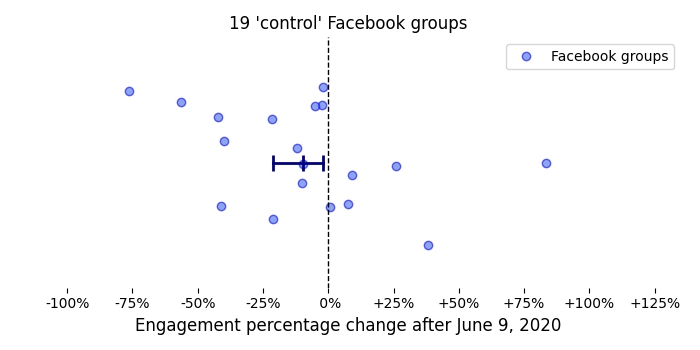
\includegraphics[scale=0.5]{./../figure/supplementary_mainstream_june_drop_percentage_change.png}
\caption{
Same metrics as on Figure 4 aggregated over the `control' Facebook accounts that published at least once during 30 days before and after June 9, 2020.
}
\label{june_drop_control}
\end{figure}

The percentage changes for their engagement per post averaged over 30 days after June 9, 2020 minus averaged over 30 days before are not significantly different from zero for groups (W = $95$, p-value = $0.32$, median = $-7\%$) and for pages (W = $27$, p-value = $1$, median = $-6\%$, see Figure \ref{june_drop_control}).
Contrary to what we observe for the `repeat offender' groups, we observe no drop in engagement in June 2020 for the `control' groups.
This confirms that the drop observed for the `repeat offender' groups is specifically targeted at them, and is not a feature that broadly affected Facebook accounts.

\section*{Overlap between the lists of false URLs}

We expect that there is an overlap between the lists of False URLs obtained from the Science Feedback and the Condor datasets. 
Indeed, Science Feedback is a third-party fact-checker partnering with Facebook \citep{sciencefeedbackFbPartner}, and communicates URLs to be flagged as false to Facebook.
However the Condor dataset only contains URLs that have been shared by more than 100 users on Facebook, and excludes the least viral ones.
As Condor is one of the largest social science research dataset ever constructed, issues related to data quality, validity and fidelity are expected \cite{messing2020facebook}, which argues in favour of using partially redundant datasets as done in this study.
For example, it was recently revealed that demographics data in Condor were only based on about half of the U.S. users for which Facebook could classify their political views \citep{NYTrevelations}. 
Although this error should not impact the list of URLs we used in this article, other issues might affect the integrity of the list of False URLs obtained from this dataset.

To compare the two lists of URLs, we first standardized the format of all the URLs with the same method (stripping them of usually non-discriminant parts such as irrelevant query items or sub-domains etc), and then built a Venn diagram from the two lists of normalized URLs (see Figure \ref{venn_urls}). 

\begin{figure}[!h]
\centering
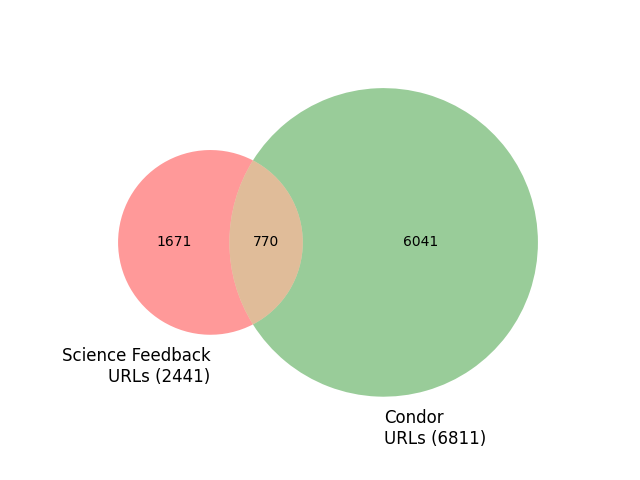
\includegraphics[scale=0.5]{./../figure/supplementary_venn_urls.png}
\caption{
Overlap between the list of False URLs from Science Feedback and the list of False URLs from Condor.
}
\label{venn_urls}
\end{figure}

We observe a moderate overlap, with $32\%$ of the URLs in Science Feedback data that are also found in Condor, suggesting that most of the URLs fact-checked by Science Feedback were shared by less than 100 users. 
The URLs from Science Feedback represent $11\%$ of all the ones we find in Condor.

\section*{Overlap between the different sets of accounts analyzed}

We used different data and methodologies to obtain three lists of `repeat offender' accounts and here we assess how much redundancy exists between these lists. 

\begin{figure}[!h]
\centering
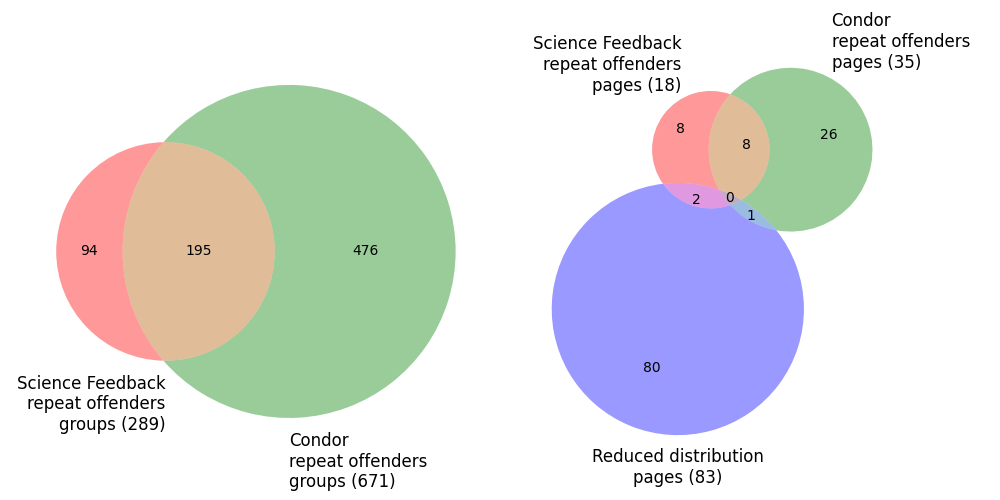
\includegraphics[scale=0.5]{./../figure/supplementary_venn_groups_and_pages.png}
\caption{
\textbf{(Left panel)} Overlap between the two lists of Facebook groups identified using Science Feedback data (first analysis) and Condor data (second analysis). \textbf{(Right panel)} Overlap between the three lists of Facebook pages identified using Science Feedback data (first analysis), using Condor data (second analysis) and using the `reduced distribution' notification approach (third analysis).
}
\label{venn_accounts}
\end{figure}

We found no groups declaring to be under ‘reduced distribution’ (third approach), and thus only compare the lists of Facebook groups collected between the first and second analyses (see Figure \ref{venn_accounts} left panel).
Although the lists of false URLs did not overlap much between the two datasets, we found that two third ($67\%$) of the groups identified using Science Feedback data were also obtained from Condor data. 
The reason for this might be that the URLs in common between the Science Feedback and Condor datasets are the most viral ones (shared by more than 100 users). 
These most viral URLs could be determinant in identifying accounts that repeatedly share misinformation.

We also compare the lists of pages found using the three different methods (Figure \ref{venn_accounts} right panel).
Again, there is a significant overlap between the page lists obtained with the two first methods, with 8 pages out of the 18 identified using Science Feedback data that were also found using Condor data.
The overlap between the two first lists and the 83 pages sharing a `reduced distribution' notification was almost null (with only 2 pages in common with the first list, and 1 page with the second list).
The `reduced distribution' notifications used to identify the last set of pages were mostly shared during the last semester of 2020.
Because we selected only the pages that shared 24 or more False URLs in the two first analyses, it is possible that this approach selected pages that received their first `reduced distribution' notification in 2019 or earlier in 2020.
This would explain the small overlap between pages identified as having shared False URLs and pages identified as having shared a `reduced distribution' notification.

The fact that we obtained different sets of pages further argues in favour of using a variety of approaches to investigate the effects of the `repeat offender' policy.

\bibliography{mybibfile}


\end{document}
